\scanpage{17}
% Upper continuation and insertion.
\inserted{\unsure{provenant de}} l'isom canonique entre $X\times Y$ et $Y\times X$. Soit alors
\[
\varphi^*=s\varphi^\circ:\mathcal V^\circ\longrightarrow\mathcal V^A.
\]
on \unsure{constate} alors que le composé
\[
\psi\varphi^*=\psi(s\varphi^\circ)=(\psi s)\varphi^\circ:\mathcal V^\circ\longrightarrow k\text{-mod gr}
\]
est \deleted{\unsure{donc}} \uline{égal} à $\omega^*A^\circ:\mathcal V^\circ\longrightarrow k\text{-mod gr}$.
\margin{\uline{vérifier}}

\deleted{Ainsi, $\mathcal V^A$ \unsure{apparaît comme une espèce d'enveloppe}}

% Middle paragraph.
\uline{Car si $\mathcal V$ a un objet final $e$, et si de plus} $A(e)=k$ \inserted{[Sinon, on remplace $k$ par $A(e)$!]} Alors les $A(X)$ sont naturellement jaugés; si c'est des Alg. de Poincaré, il suffit alors de connaître \deleted{\unsure{les}} Alg. jaugées, $+$ les $f^*$ ($f:X-Y$ de $\mathcal V$) pour connaître $A$.

Soit
\[
\begin{aligned}
u&\in\operatorname{Hom}_{\mathcal V^A}(X,Y)=A(X\times Y)\\
su&\in\operatorname{Hom}_{\mathcal V^A}(Y,X)=A(Y\times X)
\end{aligned}
\]
donc $\tilde u:A(X)\longrightarrow A(Y)\qquad\widetilde{su}:A(Y)\longrightarrow A(X)$.

Montrons que \inserted{si $u$ central dans $A(X\times Y)$, alors} $\tilde u$ et $\widetilde{su}$ sont transposés l'un de l'autre, pour les formes $\unsure{k|\kappa}_{A(X)}$ et $\unsure{k|\kappa}_{A(Y)}$ sur $A(X)$, $A(Y)$, i.e.\ on a pour $x\in A(X)$, $y\in A(Y)$, $u\in A(X\times Y)$
\[
\unsure{k|\kappa}_Y\bigl(y\unsure{\tilde u_*(x)|u_*(x)}\bigr)=\unsure{k|\kappa}_X\bigl(\unsure{\tilde u^*(y)|u^*(y)}x\bigr)\qquad\text{i.e.}
\]
\[
g_*(y u_*(x))=f_*(u^*(y)x).\quad(\uuline{\text{Car $u$ central!}})\quad\text{En effet}
\]
\margin{$\unsure{g^*}$}
\diagram{\begin{tikzcd}
A(X)\arrow[r,shift left,"u_*"]\arrow[d,"\unsure{k|\kappa}_X"'] & A(Y)\arrow[l,shift left,"u^*"]\arrow[d,"\unsure{k|\kappa}_Y"]\\
k\arrow[r,phantom,"="]&k
\end{tikzcd}}
\diagram{\begin{tikzcd}
&X\times Y\arrow[dl,no head,"p_1"']\arrow[dr,no head,"p_2"]&\\
X\arrow[dr,no head,"f"']&&Y\arrow[dl,no head,"g"]\\
&e&
\end{tikzcd}}
\[
\begin{aligned}
g_*(y u_*(x))
&=\unsure{g_*}\bigl(y p_{2*}(u p_1^*(x))\bigr)
=g_*p_{2*}(p_2^*(y)u p_1^*(x))
=\unsure{k(p_2^*(y)u p_1^*(x))}\\
f_*(u^*(y)x)
&=f_*\bigl(p_{1*}(u p_2^*(y))x\bigr)
=f_*p_{1*}(u p_2^*(y)p_1^*(x))
=k(u p_2^*(y)p_1^*(x))\\
&\unsure{\geq|=}\ k(p_2^*(y)u p_1^*(x))
\end{aligned}
\]
\margin{$\boxed{\text{mod. signe!}}$}
\figure{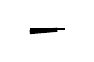
\begin{tikzpicture}\draw[line width=1.5pt] (0,0)--(.35,.03);\draw (0,.04)--(.45,.04);\end{tikzpicture}}
\mspage{16}
